O método de Interpolação Polinomial é mais um método numérico iterativo para minimização de funções unidimensionais. 
O mesmo consiste em interpolar polinômios de segundo grau ($ax^2+bx+c$) a partir de 3 pontos da função, e achar o ponto mínimo dessa curva interpolada. 

Digamos que queremos minimizar a função mostrada na figura \ref{fig:interpol_1}, escolhem-se dois pontos que definem um intervalo onde sabe-se previamente que possui um mínimo, na figura $x_1$ e $x_3$, o ponto $x_2$ é escolhido na metade do intervalo. A partir destes pontos encontra-se o valor da função nesses pontos e resolve-se o sistema $A\vec{x}=\vec{b}$, onde A é a matriz com os valores $x^2$, $x$ e $1$ para cada valor de x ($x_1$, $x_2$  e $x_3$), $\vec{x}$ são os valores dos coeficientes do polinômio interpolado e $\vec{b}$ os valores da função para cada x marcados em \ref{fig:interpol_2}.



Após interpolado, vemos a curva azul na figura \ref{fig:interpol_3} que representa a interpolação. E a partir dos coeficientes do polinômio sabemos que o mínimo encontra-se no valor em que $x=\frac{-b}{2a}$, ponto $x_4$ na figura \ref{fig:interpol_4}. Com os 4 pontos devemos escolher os três pontos que resultem no menor valor de função para prosseguir com o algoritmo. Escolhendo os pontos $x_1$, $x_2$ e $x_2$ realizamos novamente a interpolação como vemos na figura \ref{fig:interpol_5}.

Uma das coisas que podem acontecer é o valor encontrado de mínimo do polinômio interpolado, coincidir com um dos valores de x já usados, assim como acontece na figura \ref{fig:interpol_5}, uma maneira de contornar este problema é encontrar dois pontos já utilizados e recomeçar o algoritmo, neste caso podemos ver que foi escolhido o intervalo entre $x_1$ e $x_4$, em verde na mesma figura.

O algoritmo de interpolação puro é capaz de encontrar diversas dificuldades, devido a necessidade de inverter matrizes e de alguns valores de funções serem muito próximos para todos os três pontos, tornando a matriz mal condicionada. A fim de mostrar algumas dessas dificuldades, foi elaborado o algoritmo puro, sem as correções conhecidas dos métodos de Brent e afins.
\begin{figure}[H]
	\begin{center}	
		\begin{subfigure}{.5\textwidth}
  			\centering
  			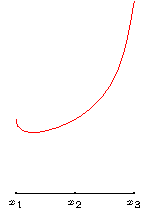
\includegraphics[width=4.5cm]{../interpol/interpol_1}
  			\caption{Função a ser minimizada}
  		\label{fig:interpol_1}
		\end{subfigure}%
		\begin{subfigure}{.5\textwidth}
  			\centering
  			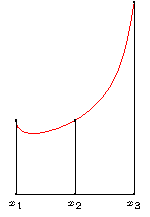
\includegraphics[width=4.5cm]{../interpol/interpol_2}
  			\caption{Valor da função em $x_1$ $x_2$ e $x_3$}
  			\label{fig:interpol_2}
		\end{subfigure}	
	\end{center}
	\caption{Aquisição dos pontos}
\end{figure}

\begin{figure}[H]
	\begin{center}	
		\begin{subfigure}{.5\textwidth}
  			\centering
  			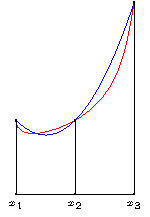
\includegraphics[width=4.5cm]{../interpol/interpol_3}
  			\caption{Curva interpolada em azul}
  		\label{fig:interpol_3}
		\end{subfigure}%
		\begin{subfigure}{.5\textwidth}
  			\centering
  			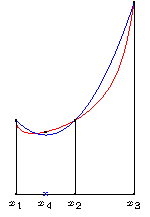
\includegraphics[width=4.5cm]{../interpol/interpol_4}
  			\caption{x do mínimo da interpolação em azul e valor da função nele}
  			\label{fig:interpol_4}
		\end{subfigure}	
	\end{center}
	\caption{Interpolação e minimização}
\end{figure}

\begin{figure}[H]
	\begin{center}		
  			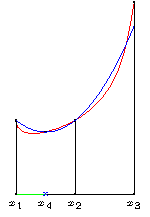
\includegraphics[width=4.5cm]{../interpol/interpol_5}
  			\caption{Segunda interpolação e próxima região para interpolação em verde}
  			\label{fig:interpol_5}
	\end{center}
\end{figure}


Depois de construído o algoritmo foram feitos testes com as mesmas funções:

\begin{itemize}
	\item $ f_1(x) = 3x^2 + 20x - 8 $
	\item $ f_2(x) = xsin(x)cos(x) $
	\item $ f_3(x) = 5x $
	\item $ f_4(x) = -e^{-\mid x \mid} $
\end{itemize}

E para fim de comparação com os outros métodos, foram usados exatamente os mesmos parâmetros, os resultados podem ser visto nas figuras de número \ref{fig:f1_gui} a \ref{fig:f4_resultados}.
\\
\begin{figure}[H]
	\begin{center}	
		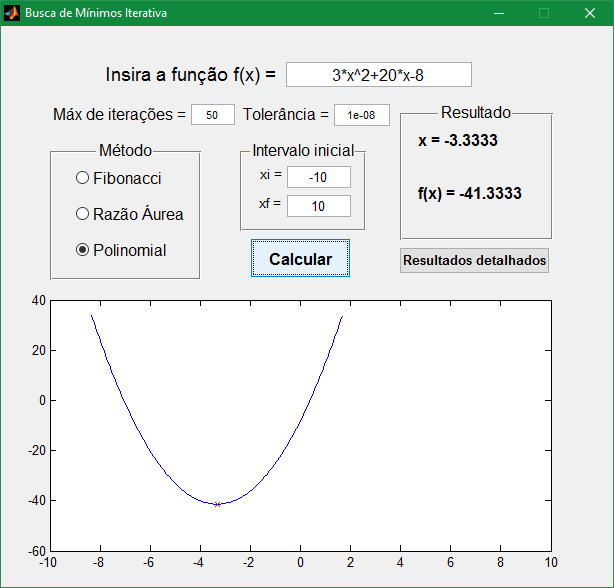
\includegraphics[width=14cm]{../interpol/f1_gui.PNG}
		\caption{Resultados para a função $f_1$}
		\label{fig:f1_gui}
	\end{center}
\end{figure}

\begin{figure}[H]
	\begin{center}	
		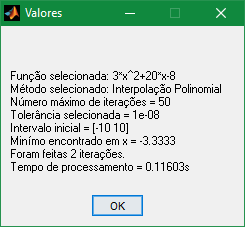
\includegraphics[width=6cm]{../interpol/f1_resultados.PNG}
		\caption{Resultados para a função $f_1$}
		\label{fig:f1_resultados}
	\end{center}
\end{figure}

\begin{figure}[H]
	\begin{center}	
		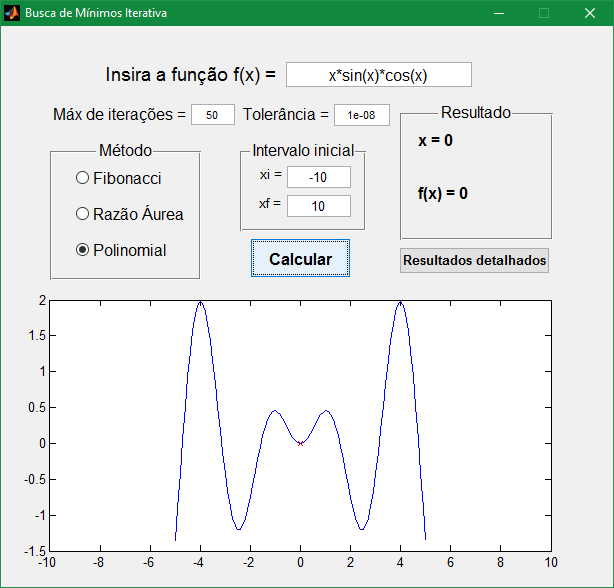
\includegraphics[width=14cm]{../interpol/f2_gui.PNG}
		\caption{Resultados para a função $f_2$}
		\label{fig:f2_gui}
	\end{center}
\end{figure}

\begin{figure}[H]
	\begin{center}	
		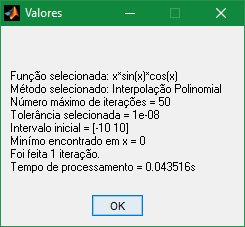
\includegraphics[width=6cm]{../interpol/f2_resultados.PNG}
		\caption{Resultados para a função $f_2$}
		\label{fig:f2_resultados}
	\end{center}
\end{figure}

\begin{figure}[H]
	\begin{center}	
		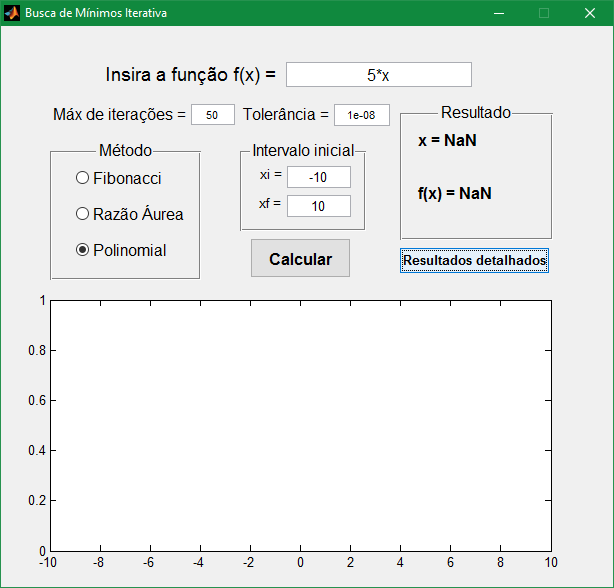
\includegraphics[width=14cm]{../interpol/f3_gui.PNG}
		\caption{Resultados para a função $f_3$}
		\label{fig:f3_gui}
	\end{center}
\end{figure}

\begin{figure}[H]
	\begin{center}	
		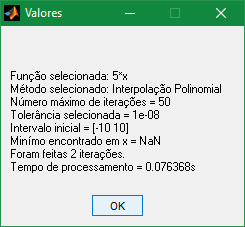
\includegraphics[width=6cm]{../interpol/f3_resultados.PNG}
		\caption{Resultados para a função $f_3$}
		\label{fig:f3_resultados}
	\end{center}
\end{figure}



\begin{figure}[H]
	\begin{center}	
		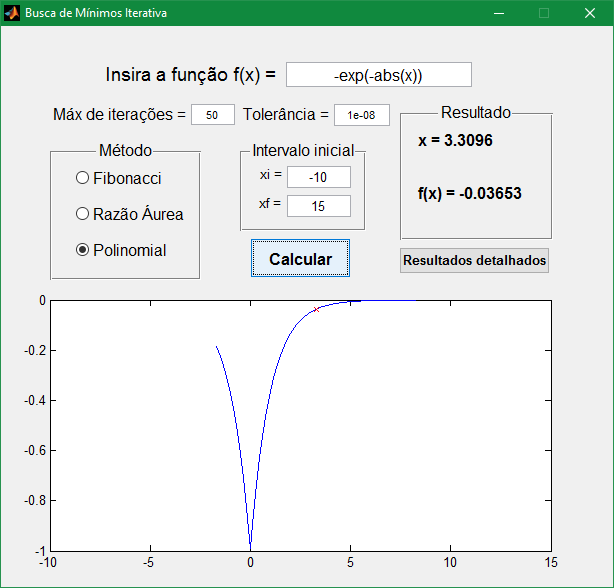
\includegraphics[width=14cm]{../interpol/f4_gui.PNG}
		\caption{Resultados para a função $f_4$}
		\label{fig:f4_gui}
	\end{center}
\end{figure}

\begin{figure}[H]
	\begin{center}	
		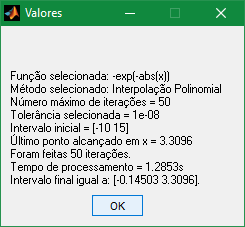
\includegraphics[width=6cm]{../interpol/f4_resultados.PNG}
		\caption{Resultados para a função $f_4$}
		\label{fig:f4_resultados}
	\end{center}
\end{figure}

